\documentclass[12pt,letter]{article}
\usepackage{xcolor}
\usepackage[top=2cm, bottom=2cm, left=2cm, right=2cm, headsep=2mm, foot=4mm]{geometry}
\usepackage{amsmath,amsthm,amsfonts,amssymb,amscd}
\usepackage{enumerate}
\usepackage{parskip}
\usepackage{mathtools}
\usepackage{mathrsfs}
\usepackage{mdframed}
\usepackage{graphicx}
\graphicspath{ {./img/} }

\title{Homework 1 - AMATH 583}
\author{Warren Paris-Moe}
\date{April 2023}

\begin{document}

\section{Problem 1}
\begin{mdframed}
Write a C or C++ program that finds a practical measure of your machine’s SP (32 bit) and DP (64 bit)
precision by taking the difference of 2 numbers and comparing the result to zero in each data type. You
will submit the code, and in the written homework will state the values you obtained running your code
for each data type. Use a while loop and iterate over $j = 0, 1,...$. 
Hint: while $((1-(1+\frac{1}{2^j})\neq0)$ \{... j++;\}
\end{mdframed}

The results of the machine epsilon estimate are as follows:
\begin{itemize}
    \item Single-Precision (SP) Precision: 5.960464478e-08
    \item Double-Precision (DP) Precision: 1.110223025e-16
\end{itemize}

\section{Problem 2}
\begin{mdframed}
What are the largest and smallest SP (32 bit) and DP (64 bit) numbers that can be represented in IEEE
arithmetic? Show your work as this is analytic.
\end{mdframed}

\textbf{IEEE:} $V = (-)^S * M * 2^E$ where $S$ is the sign bit, $M$ are the $n$ significand/mantissa bits, and $E$ is the $k$ bit exponent field. $S$ is always 1-bit while the exponent and mantissa bits vary depending on the precision level. $M$ is represented as a fraction $1+f$ where $f=f_{n-1}f_{n-2}...f_0$ with the exponent $e_{k-1}e_{k-2}...e_0$ which shifts the fraction, or mantissa number.

\subsection{Single Precision}
For a single precision (32 bit) number represented in IEEE, the exponent has $k=8$ bits and the mantissa is $n=23$ bits long. Along with the single sign bit, this totals to 32 bits for a single precision number. \\

We can calculate the largest positive number that can be represented in single precision by setting all exponent and mantissa bits to 1 with a sign bit of 0 (Note: the exponent $11111111_2$ is reserved for NaNs and infinity in the normalized case). The smallest is found by setting the sign bit to 1 to make the number negative. Thus, our largest and smallest single precision numbers are respectively
\begin{align*}
    & 0\:11111110\:11111111111111111111111_2, \\
    & 1\:11111110\:11111111111111111111111_2
\end{align*}
Converting the first of these to decimal we have 
\begin{align*} 
    V &= (-)^0 * (1+(1-2^{-23})* 2^{2^{8-1} - 1} \\
    &= (2-2^{-23} * 2^{2^7 - 1} \\
    &= \mathbf{3.4028*10^{38}}
\end{align*}
Doing this similarly for the smallest single precision number we get $\mathbf{V = −3.4028*10^{38}}$ in decimal.

\subsection{Double Precision}
Now for a double precision number represented in IEEE format we have 1 sign bit, $k=11$ exponent bits, and $n=52$ mantissa fraction bits totalling to 64 bit number. We follow the same procedure as before by setting all exponent bits to 1 except for the last with all mantissa bits equal to 1. The sign bit makes the distinction between the largest and smallest double precision numbers as follows:
\begin{align*}
    & 0\:11111111110\:111111111111111111111111111111111111111111111111111_2, \\
    & 1\:11111111110\:111111111111111111111111111111111111111111111111111_2
\end{align*}
Converting the first of these to decimal we have 
\begin{align*} 
    V &= (-)^0 * (1+(1-2^{-52})* 2^{2^{11-1} - 1} \\
    &= (2-2^{-52} * 2^{2^10 - 1} \\
    &= \mathbf{1.7977*10^{308}}
\end{align*}
Doing this similarly for the smallest double precision number we get $\mathbf{V = −1.7977*10^{308}}$ in decimal.


\section{Problem 3}
\begin{mdframed}
Write a C or C++ program to multiply the integers 200*300*400*500 on your computer? What is the
result? You will submit the code, and in the written homework will name the effect you observed AND
provide a definition and math formula for \textit{underflow} and \textit{overflow} for IEEE SP and DP representations.
\end{mdframed}

The effect of multiplying the integers 200*300*400*500 on my computer is that the result is the following error message:
\begin{itemize}
    \item warning: integer overflow in expression of type ‘int’ results in ‘-884901888’ [-Woverflow]
\end{itemize}
Underflow and overflow are two possible errors that can occur when working with out-of-range floating-point numbers in a computer. Underflow occurs when a result is too small to be represented by the chosen format, and it becomes rounded to zero. Overflow occurs when a result is too large to be represented by the chosen format, and it becomes rounded to infinity or the maximum representable value.
The math formula for underflow is: $x < 2^{-t+1}$, where x is the magnitude of the number and t is the number of bits used to represent the exponent.

\section{Problem 4}
\begin{mdframed}
How many SP (32 bit) normalized floating point numbers are there? Same question for DP (64 bit).
Provide a math formula and show your work.
\end{mdframed}

A IEEE floating point number is constructed by the formula $V = (-)^S M 2^E$ where $S$ is the single
sign bit $s$, $M$ is the $n$ mantissa bits, and $E$ is the $k$ exponent bits. Therefore, to find all 
possible combinations of floating point numbers we must calculate the number of permutations for each
of the three compnents.

\subsection{Single Precision}
For single precision we have $s=1$, $k=8$, and $n=23$. The number of permutations for each of these is
$2^1$ possibilities for the sign bit, $2^{23}$ for the mantissa, and $2^8$ for the
exponent (All 1s and all 0s are reserved for special cases). Thus, together we have
\begin{align*}
    \text{\# of SP permutations} &= 2^1 2^{23} (2^8 - 2) \\
    &= 2^{24}(2^8 - 2) \\
    &= 2^{32} - 2^{25} \\
    &= 4,261,412,864
\end{align*}

\subsection{Double Precision}
For double precision we have $s=1$, $k=11$ exponent bits, and $n=52$ mantissa bits. Note that we 
still have the special cases for the exponent. Thus, our total number of double precision floating 
point numbers is given by
\begin{align*}
    \text{\# of DP permutations} &= 2^1 2^{52} (2^{11} - 2) \\
    &= 2^{53} (2^{11} - 2) \\
    &= 2^{64} - 2^{54} \\
    &= 1.8428*10^{19}
\end{align*}

\subsection{Formula}
The general formula for the total number of floating point numbers for a given precision level is
$2^{s} 2^n (2^k - 1)$ where $s$ is the number of sign bits, $n$ is the number of mantissa bits, and 
$k$ is the number of exponent bits. Since $s=1$ for all IEEE floating point representations, this 
simplifies to $\mathbf{2^{n+k+1} - 2^{n+2}}$. Note that $n+k+1$ is equal to the total number of bits 
used in the IEEE representation of the floating point number. 

\section{Problem 5}
\begin{mdframed}
Consider a 6 bit floating point system with one sign bit ($s=1$), a 3-bit exponent ($k=3$), and a 2-bit
mantissa ($n=2$). Enumerate by hand all the representable normalized and denormalized numbers. Plot
the distribution of the representable numbers on a line.
\end{mdframed}

\[
    V = (-)^S (1 + f) 2^{e - bias}
\]
where $e=e_2e_1e_0$, $f=f_1f_0$, and $\text{bias}=2^{k-1} - 1 = 2^{3-1}-1 = 3$.

\subsection{Normalized}

\subsubsection{Exponent}
The exponent has $2^3=8$ possible variations which are shown below. Here $E_{e_2e_1e_0} = e_2e_1e_0 - \text{bias}$.
\begin{table}[h]
\centering
\begin{tabular}{l|l|l|l}
    $e=e_2e_1e_0$ & Decimal Conversion          & $\mathbf{E_{e_2e_1e_0}}$ & Note                                      \\ \hline
    000           & $0*2^2 + 0*2^1 + 0*2^0 = 0$ &                               & (Reserved for $\pm0.0$)                              \\
    001           & $0*2^2 + 0*2^1 + 1*2^0 = 1$ & $1-3=-2$                      &                                                      \\
    010           & $0*2^2 + 1*2^1 + 0*2^0 = 2$ & $2-3=-1$                      &                                                      \\
    011           & $0*2^2 + 1*2^1 + 1*2^0 = 3$ & $3-3=0$                       &                                                      \\
    100           & $1*2^2 + 0*2^1 + 0*2^0 = 4$ & $4-3=1$                       &                                                      \\
    101           & $1*2^2 + 0*2^1 + 1*2^0 = 5$ & $5-3=2$                       &                                                      \\
    110           & $1*2^2 + 1*2^1 + 0*2^0 = 6$ & $6-3=3$                       &                                                      \\
    111           & $1*2^2 + 1*2^1 + 1*2^0 = 7$ &                               & ($\pm \infty$ if $f=0$, NaN if $f\neq 0$)
\end{tabular}
\caption{\label{exp-norm} Exponent variations for the normalized case.}

\end{table}

The mantissa has $2^2=4$ variations shown in the next table in this section. Here $M_{f_1f_0} = 1 + f$.
\begin{table}[h!]
    \centering
\begin{tabular}{l|l|l}
    $f=f_1f_0$ & Decimal Conversion                                        & $\mathbf{M_{f_1f_0}}$             \\ \hline
    00         & $0*\frac{1}{2^1} + 0*\frac{1}{2^2} = 0$                   & $1+0=1$                                   \\
    01         & $0*\frac{1}{2^1} + 1*\frac{1}{2^2} = \frac{1}{4}$         & $1+\frac{1}{4}=\frac{5}{4}$                 \\
    10         & $1*\frac{1}{2^1} + 0*\frac{1}{2^2} = \frac{1}{2}$         & $1+\frac{1}{2}=\frac{3}{2}$                   \\
    11         & $1*\frac{1}{2^1} + 1*\frac{1}{2^2} = \frac{3}{4}$         & $1+\frac{3}{4}=\frac{7}{4}$                 \\
\end{tabular}
\caption{Mantissa variations for the normalized case.}
\label{tab:mant-norm}
\end{table}

\begin{figure}[h]
    \centering
    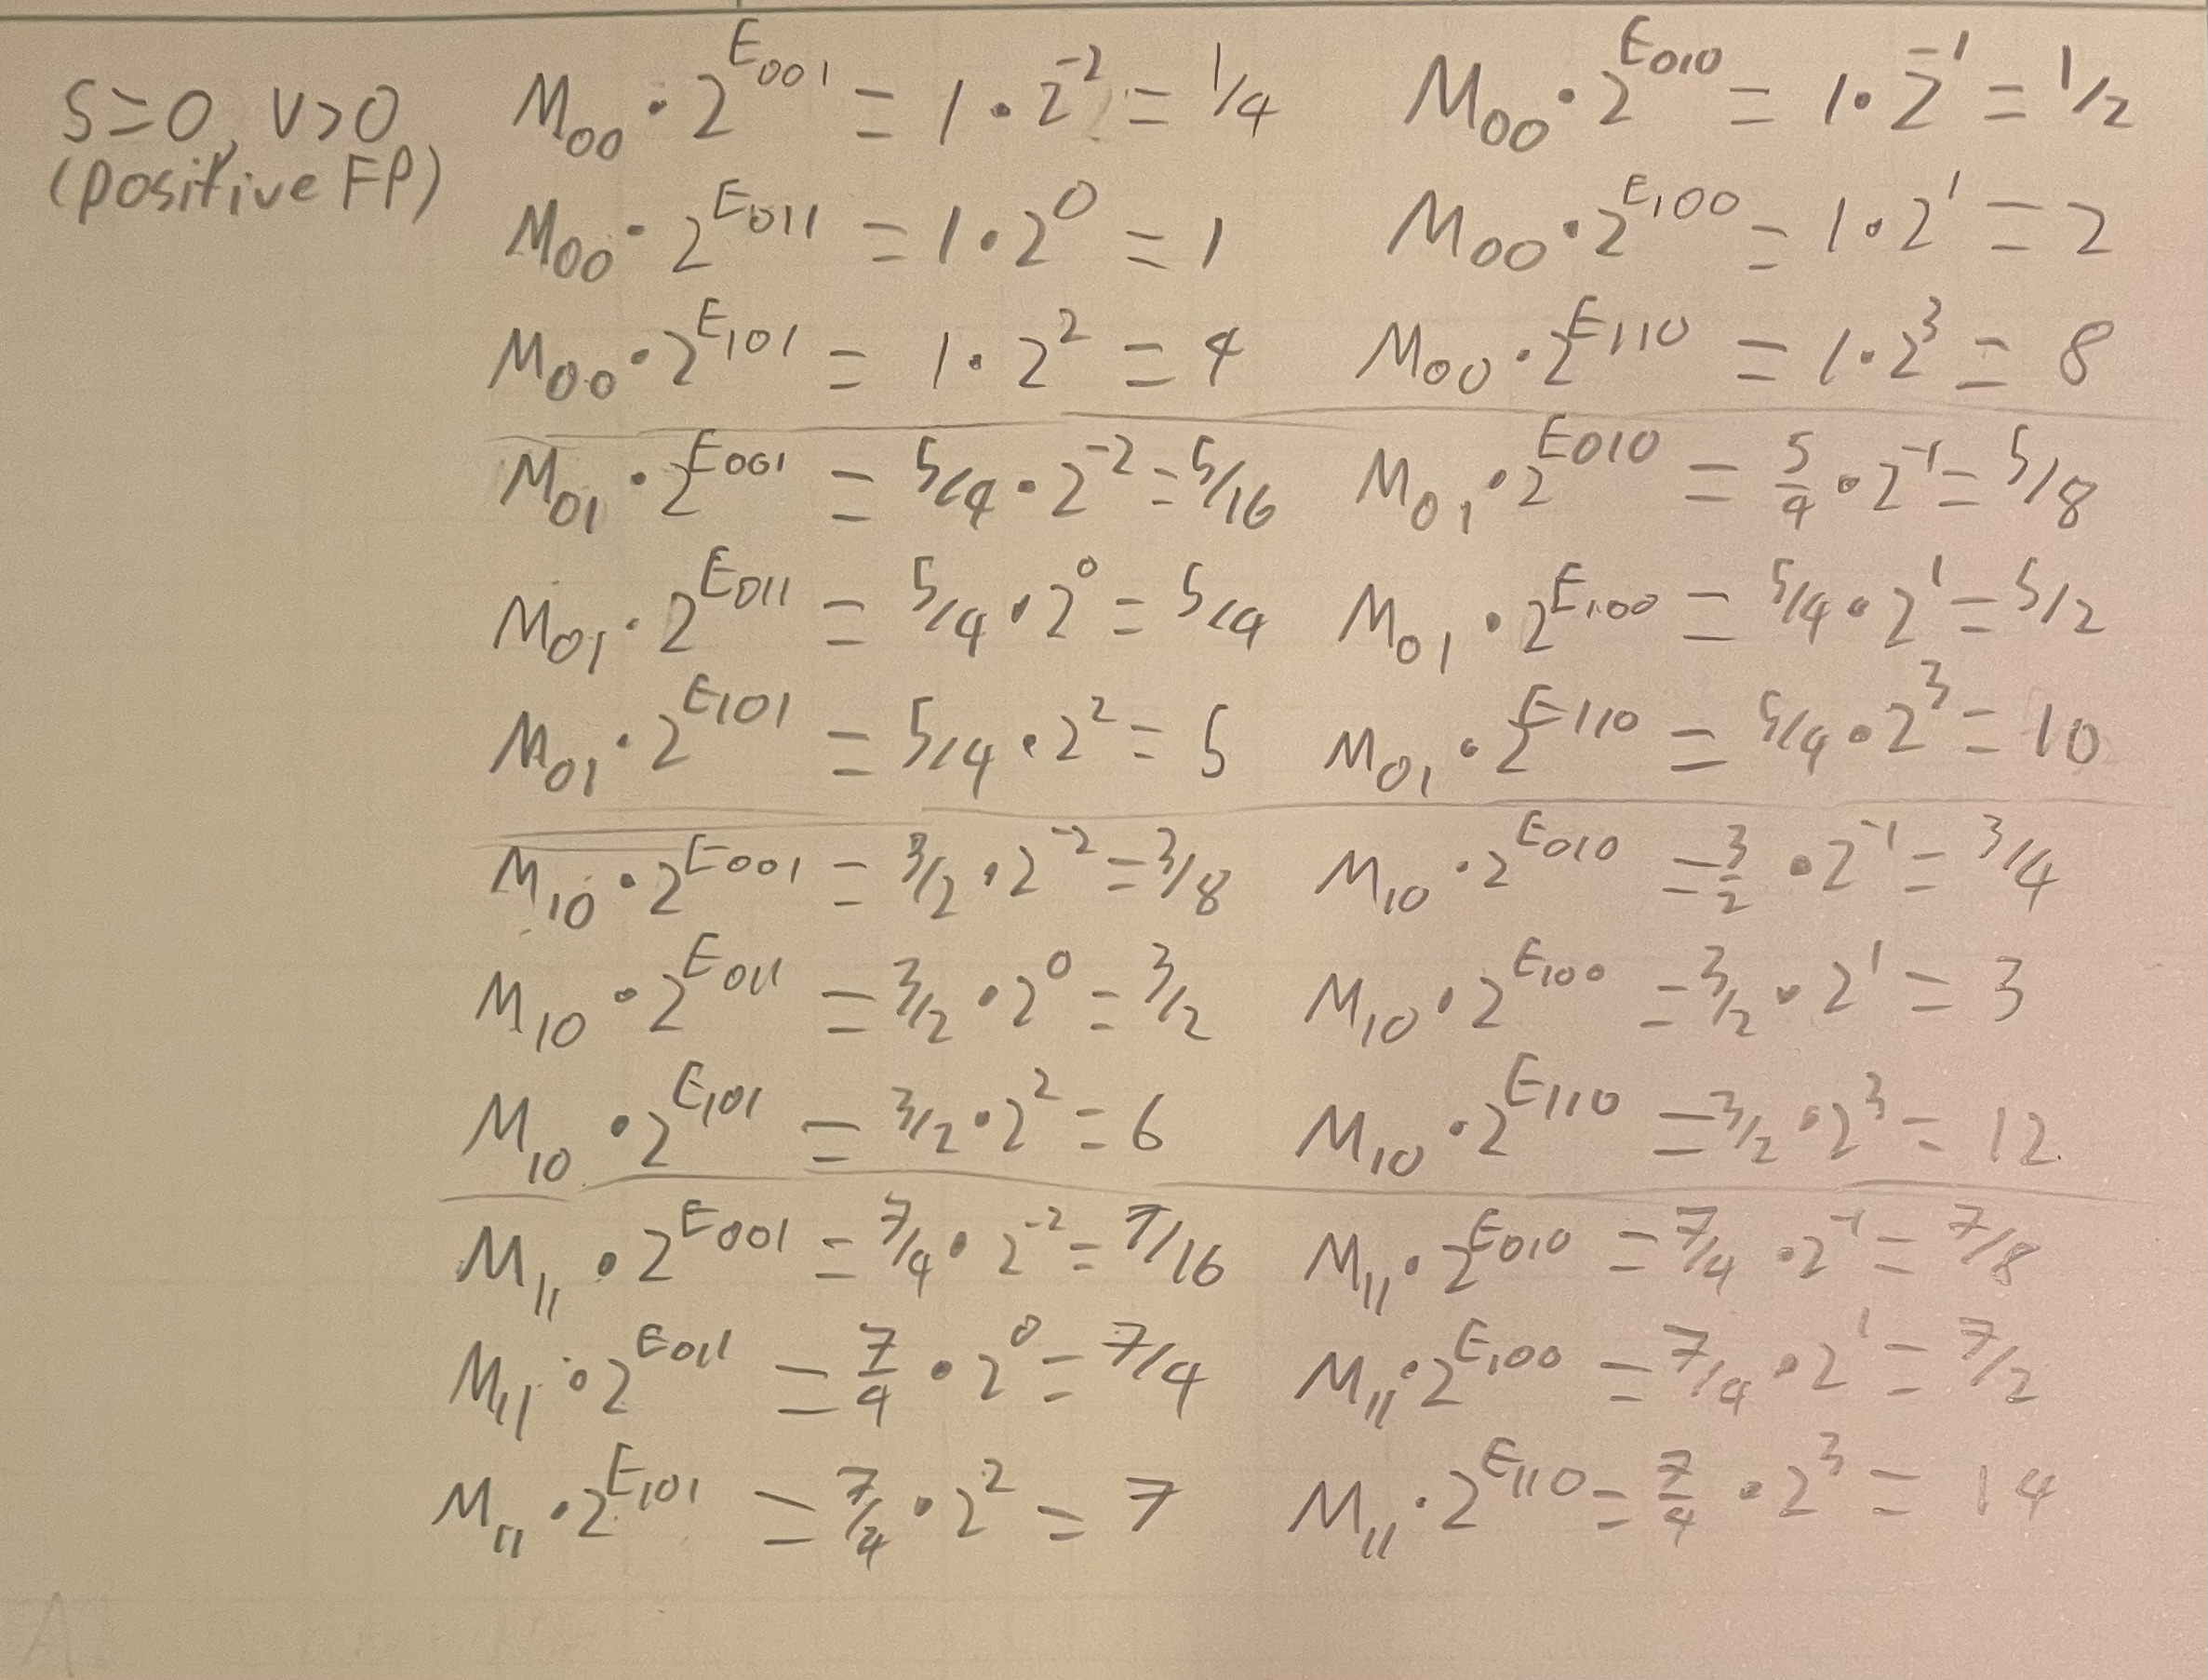
\includegraphics[scale=0.18]{pos_norm.jpg}
    \caption{Positive normalized 6-bit floating point numbers.}
\end{figure}
For the positive numbers with $s=0$ we have 24 possible normalized floating point numbers shown in the figure. 
There are 24 additional numbers for the negative numbers with $s=1$. These are the same set of numbers except with
the sign bit flipped making them negative. This totals for 48 normalized floating point numbers. The distribution 
plotted on a single number line is shown below.
\begin{figure}[h!]
    \centering
    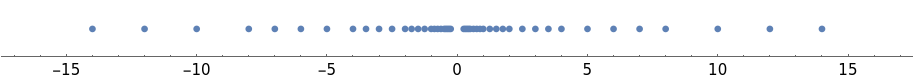
\includegraphics[scale=0.75]{numberline_norm.png}
    \caption{Distribution of representable normalized floating point numbers.}
\end{figure}


\subsection{Denormalized}
For the denormalized case, the exponent is fixed to $E=1-\text{bias}=1-3=-2$. This leaves the same 4 variationspossible for the 
fraction of the mantissa component except instead of $M=1+f$, now $M=f$. This gives us the following table.
\begin{table}[h!]
    \centering
\begin{tabular}{l|l|l}
    $M=f=f_1f_0$ & Decimal Conversion                                             \\ \hline
    00         & $0*\frac{1}{2^1} + 0*\frac{1}{2^2} = 0$                                                 \\
    01         & $0*\frac{1}{2^1} + 1*\frac{1}{2^2} = \frac{1}{4}$                  \\
    10         & $1*\frac{1}{2^1} + 0*\frac{1}{2^2} = \frac{1}{2}$         \\
    11         & $1*\frac{1}{2^1} + 1*\frac{1}{2^2} = \frac{3}{4}$        \\
\end{tabular}
\caption{Mantissa variations for the denormalized case.}
\label{tab:mant-denorm}
\end{table}

Floating point numbers in the denormalized case are represented by $V=(-)^S f 2^{1-\text{bias}}$. 
This is shown in the figure below. Note that +0.0 and -0.0 are different numbers leaving us with 8 total.
We can see that their distribution is spaced evenly shown in the figure further below.
\begin{figure}[h]
    \centering
    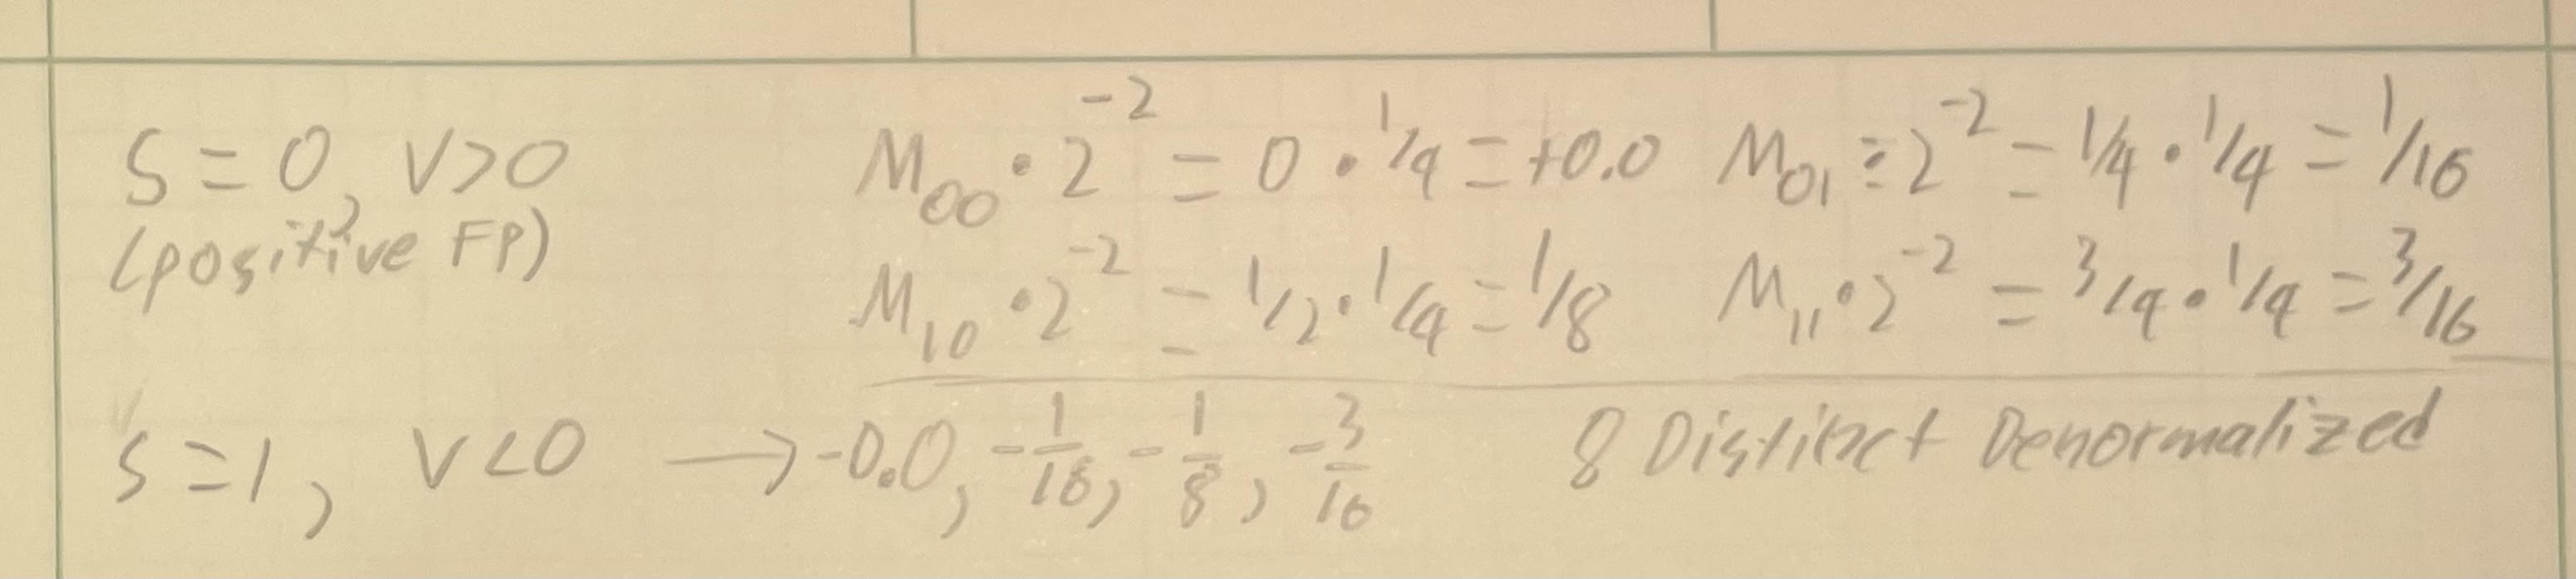
\includegraphics[scale=0.15]{denorm.jpg}
    \caption{Denormalized 6-bit floating point numbers.}
\end{figure}

\begin{figure}[h!]
    \centering
    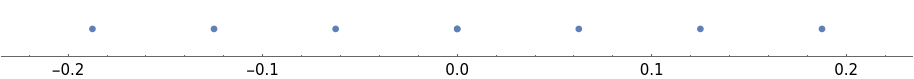
\includegraphics[scale=0.75]{numberline_denorm.png}
    \caption{Distribution of representable normalized floating point numbers.}
\end{figure}

\end{document}
